\chapter{Allgemeine Begriffe}
 
\section{Konventionen}
Bereits Rechnungen in der "`gewöhnlichen"' Relativitätstheorie haben die Tendenz
unübersichtlich zu werden, das Einführen zusätzlicher Dimensionen hilft dabei
natürlich kaum.
Es ist deshalb an dieser Stelle nützlich einige Konventionen festzulegen. Im
Folgenden bezeichnet $n$ die Anzahl der Zusatzdimensionen.\footnote{Im Weiteren
meist $n=1$}

Die Metrik soll stets die Signatur $(1,3)$, bzw. $(1,3+n)$, insbesondere sind
die Zusatzdimensionen. Die meisten Rechnungen werden in lokalen Koordinaten
durchgeführt.
Wir beginnen die Indizierung bei 0, wobei die 0. Komponente mit der Zeit identifiziert wird.
Griechische Indices laufen über ersten vier Raum-Zeit Koordinaten
$\mu=0,\ldots,3\,$, lateinische über alle inklusive der
Zusatzkomponenten \footnote{Verwirrung bezüglich der gängigen Konvention
mit lateinischen Indices die Raumkomponenten zu benennen sollte dabei nicht
aufkommen.}, $i=0,\ldots,3+n\,$. Weiter verwenden wir die Einsteinsche
Summenkonvention, d.h. über paare von indices wird implizit summiert.

Im Zusammenhang mit Zusatzdimensionen tauchen Größen auf, die sowohl ein 4, als
auch ein $4+n$ dimensionales Pendant besitzen. Um diese von einander zu
unterscheiden, kennzeichnen wir die $4+n$ dimensionale Version mit einem
Zirkumflex. 
Beispielsweise bezeichnen wir den $4+n$ dimensionalen Ricci-Tensor mit
$\tensor{\hat{R}}{_i_j}$. Mit $g$ bezeichnen wir die Determinante der Metrik.
\subsection*{Geometrisierte Einheiten}
Wir verwenden geometrisierte Einheiten, d.h. Einheiten in denen
$8\pi G=c=1$. Es verbleibt nur noch eine Längendimension.
\section{Differentialgeometrie}
Wir wollen Manigfaltigkeiten betrachten, welche gewisse Symmetrien besitzen.
Anschaulich beschreibt eine Symmetrie die Invarianz eines Objektes unter einer
Operation.
Ein einfaches Beispiel für eine solche Symmetrie stellt der Zylinder
\begin{equation}
Z=\Reals\times\Sphere^1=\left\{(x,y,z)\in\Reals^3\,\Big|\,x^2+y^2=1\right\} 
\end{equation}
dar. Offensichtlich kann wird dieser durch Drehung um die $z$-Achse in sich
selbst überführt. 
Wir werden uns auf bestimmte Symmetrien beschränken, die
beispielsweise infinitisimal erzeugt werden können, dies schließt Spiegelungen
und andere diskrete Symmetrien aus.
Wir wollen dieses Konzept nun etwas formalisieren. Der Zylinder dient dabei als
Anschauungsobjekt um die abstrakten Begriffe zu veranschaulichen.
\subsection{Vektoren und Tensoren}
Riemann-Tensor, Ricci-Tensor, Geodätische.
\subsection{Gruppenwirkungen}
\subsection{Lie-Gruppen}
Eine Lie-Gruppe ist eine Gruppe, die zusätzlich eine Differenzierbare Struktur
besitzt.
In unserem Fall ist die Lie-Gruppe die die Operationen beschreibt die Gruppe der
Drehungen um die $z$-Achse. Diese wird mit $SO(2)$ bezeichnet, eine Darstellung
ergit sich beispielsweise durch Matrizen der Form
\begin{equation}
R(\alpha)=
\begin{pmatrix}
\cos\alpha&\sin\alpha&0\\
-\sin\alpha&\cos\alpha&0\\
0&0&1
\end{pmatrix}
\end{equation}
Das diese Gruppe eine differenzierbare Struktur besitz ist klar da die
Komponenten der Matrizen differenzierbar sind.
\begin{definition}[Lie Gruppe]

\end{definition}

Gruppen können auf Mengen operieren.  Um die Diskussion allgemeiner zu gestalten definieren wir
Operationen allgemeiner Gruppen. Die Hauptforderung an die Wirkung der Gruppe
auf der Menge ist, dass die Operation mit der Gruppenoperation kompatibel ist.
 \begin{definition}[Gruppenwirkung]
Sei $G$ eine Gruppe, $X$ eine Menge. Eine Abbildung
\begin{equation}
\Phi:G\times X\to X\,,\quad (g,x)\mapsto\Phi_g(x)
\end{equation}
heißt \emph{Gruppenwirkung} von $G$ auf $X$, falls die folgende Eigenschaften
erfüllt sind
\begin{enumerate}
  \item \emph{Identität}: für das neutrale Element $e\in G$ gilt
  $\displaystyle\Phi_e=\id_X$
  \item \emph{Verträglichkeit}: $\displaystyle\Phi_{gh}=\Phi_g\circ\Phi_h$
\end{enumerate}
$X$ heißt dann auch $G$-Menge.
\end{definition}
 Statt $\Phi_g(x)$ schreiben wir im folgenden kurz $g\gmal x$.
Ist die Gruppe $G$ eine Lie-Gruppe, $X=M$ eine Mannigfaltigkeit und $\Phi_g$
 glatt, so spricht man von einer \emph{Lie-Gruppenwirkuqng}. $M$ heißt dann auch
 $G$-Mannigfaltigkeit.
 \begin{definition}
 Sei $X$ eine $G$-Menge. Die Wirkung von $G$ heißt:
 \begin{enumerate}
   \item \emph{eigentlich}, falls unter der Abbildung $\Gamma_G:(g,x)\mapsto (g
   \gmal x,x)$, Urbilder kompakter Mengen kompakt sind
   \item \emph{(fixpunkt-)frei}, falls nur die Identität Fixpunkte besitz, d.h.
   $g\gmal x=x$, impliziert $g=e$.
 \end{enumerate}
 \end{definition}
 \begin{beispiel}[Wirkung von $\Reals/\mathbb{Z}$ auf einem Zylinder]
Sei $G=(\Reals/\mathbb{Z},+)$, $Z$ wie oben. Eine Wirkung von $G$ auf $Z$ ist
erklärt durch
\begin{equation}
t.\vec{x}= \begin{pmatrix}
\cos\left( 2\pi t\right)&\sin\left( 2\pi t\right)&0\\
-\sin\left( 2\pi t\right)&\cos\left( 2\pi t\right)&0\\
0&0&1
\end{pmatrix}\vec{x}\,.
\end{equation}
Wie man sich leicht klar macht ist die Wirkung glatt, frei und eigentlich sowie 
$Z$ eine $G$-Manigfaltigkeit.
%TODO eigentlich?
\end{beispiel}
\begin{figure}
\centering
\begin{tikzpicture}
\draw[-latex] (2,1)-- (-2,-1)  ;
\draw[-latex]  (-2,1)--(2,-1)  ;

 \draw[fill=white,draw=none] (-1,4) -- (-1,0) arc (180:360:1cm and 0.5cm) -- (1,4) arc (-180:0:-1cm and 0.5cm) ;
\draw[fill=white,draw=none] (0,4) ellipse (1cm and 0.5cm);
\draw[-,thick, dashed] (0,-0.5) -- (0,4) ;
\draw[dashed] (2,1)-- (-2,-1)  ;
\draw[dashed]  (-2,1)--(2,-1)  ;
\draw[-,thick] (0,-1) -- (0,-0.5) ;
\node at (0,0) {\tiny\textbullet};
\node at (0,4) {\tiny\textbullet};
  \draw[densely dashed] (-1,2) arc (180:0:1cm and 0.5cm);

  \draw[fill=gray,fill opacity = 0.1,draw=none] (0,4) ellipse (1cm and 0.5cm);
 
  \draw[fill=gray,fill opacity = 0.2] (-1,4) -- (-1,0) arc (180:360:1cm and 0.5cm) -- (1,4) arc (-180:0:-1cm and 0.5cm) ;
  \draw[densely dashed] (-1,0) arc (180:0:1cm and 0.5cm);
  \draw(-1,4) arc (180:0:1cm and 0.5cm);

  \draw[densely dashed]  (-1,2) arc (-180:0:1cm and 0.5cm);
  \draw[thick, red, -latex] (0,2) [partial ellipse=-60:-140:1cm and 0.5cm];
 %\draw[thick, blue!80!black,-latex] (0.51,1.57)-- (0.51,3);
  \node at (2,4) {$\mathbb{R}\times\mathbb{S}^1$};
  \node at (2+0.3,-1-0.2) {$y$};
  \node at (-2+0.3,-1-0.2) {$x$};
  \node at (0.3,5) {$z$};
   \node at (0.5,1.25) {$p$};
  \draw[-latex,thick] (0,4) -- (0,5) ;
  \node at (0.51,1.57){\textbullet};
;\end{tikzpicture}
\caption{Wirkung von $\Reals/\mathbb{Z}$ auf dem Zylinder $Z$.}
\end{figure}

 \subsection{Orbiträume}
\begin{definition}[Orbit]
Sei $X$ eine $G$-Menge, $x\in X$, dann heißt die Menge
\begin{equation}
G \gmal x=\{g \gmal x\,|\,g\in G\}
\end{equation}
Orbit von $x$.
\end{definition}
Als \emph{Orbitraum} bezeichnen wir den Quotienten $M/G$ einer
$G$-Mannigfaltigkeit $M$
\begin{equation}
M/G=\{[x]=G.x|x\in M\}\,.
\end{equation}
Dieser lässt sich mit einer natürlichen Quotiententopologie $\tau$ ausstatten,
die die gröbste Topologie ist, für die die kanonische Projektion $x\mapsto [x]$
stetig ist.
\begin{beispiel}
Wenn wir wieder das Beispiel $G=\Reals/\mathbb{Z}$, $M=Z$ heranziehen, so sind die Orbits gegeben durch 
\begin{equation}
G.(0,0,z)=\left\{(\sin (2\pi t),\sin (2\pi t),z)\,,t \in
[0,1)\right\}\cong\Sphere^1\,.
\end{equation}
Der Orbitraum $M/G$ ist diffeomorph zu $\mathrm{R}$. Der Zylinder lässt sich
also lokal als Produkt von Orbitraum und Orbit darstellen.
\end{beispiel}
\begin{figure}
\centering
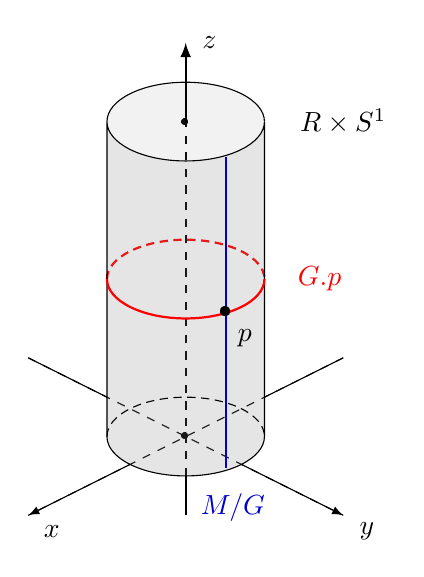
\begin{tikzpicture}
\draw[-latex] (2,1)-- (-2,-1)  ;
\draw[-latex]  (-2,1)--(2,-1)  ;

 \draw[fill=white,draw=none] (-1,4) -- (-1,0) arc (180:360:1cm and 0.5cm) -- (1,4) arc (-180:0:-1cm and 0.5cm) ;
\draw[fill=white,draw=none] (0,4) ellipse (1cm and 0.5cm);
\draw[-,thick, dashed] (0,-0.5) -- (0,4) ;
\draw[dashed] (2,1)-- (-2,-1)  ;
\draw[dashed]  (-2,1)--(2,-1)  ;
\draw[-,thick] (0,-1) -- (0,-0.5) ;
\node at (0,0) {\tiny\textbullet};
\node at (0,4) {\tiny\textbullet};
  \draw[densely dashed,red,thick] (-1,2) arc (180:0:1cm and 0.5cm);

  \draw[fill=gray,fill opacity = 0.1,draw=none] (0,4) ellipse (1cm and 0.5cm);
 
  \draw[fill=gray,fill opacity = 0.2] (-1,4) -- (-1,0) arc (180:360:1cm and 0.5cm) -- (1,4) arc (-180:0:-1cm and 0.5cm) ;
  \draw[densely dashed] (-1,0) arc (180:0:1cm and 0.5cm);
  \draw(-1,4) arc (180:0:1cm and 0.5cm);

  \draw[red,thick]  (-1,2) arc (-180:0:1cm and 0.5cm);
 % \draw[thick, red, -latex] (0,2) [partial ellipse=-60:-140:1cm and 0.5cm];
 \draw[thick, blue!80!black] (0.51,-0.4)-- (0.51,3.55);
  \node at (2,4) {$\mathbb{R}\times\mathbb{S}^1$};
  \node[red] at (1.7,2) {$G.p$};
  \node[ blue!80!black] at (0.6,-0.9) {$M/G$};
  \node at (2+0.3,-1-0.2) {$y$};
  \node at (-2+0.3,-1-0.2) {$x$};
  \node at (0.3,5) {$z$};
   \node at (0.75,1.25) {$p$};
  \draw[-latex,thick] (0,4) -- (0,5) ;
  \node at (0.51,1.57){\textbullet};
;\end{tikzpicture}
\end{figure}
% \begin{figure}
% \centering
% \begin{tikzpicture}
% 
%    \draw[dashed] (1.3,-1.33) [partial ellipse= 90:270:0.5cm and 1cm];
%    \draw[dashed] (-1.3,-1.33) [partial ellipse=90:-90:0.5cm and 1cm];
%    \draw[thick, red,dashed] (-0,-1.5) [partial ellipse=270:90:0.4cm and 1cm];
%    \node[fill=white] at (0.7,-1.2) {$p$};
%   \node at (0.4,-1.5){\textbullet};
%    \node at (1.8,-1.3){\textbullet};
%    \node at (-1.8,-1.3){\textbullet};
% \fill[fill=gray,fill opacity = 0.2]  (-3.5,0) -- (0, 2.5)  -- (3.5,0);
% \fill[fill=gray,fill opacity = 0.2]  (-3.5,0) -- (0, -2.5)  -- (3.5,0);
% \draw[fill=gray,fill opacity = 0.2] (-3.5,0) .. controls (-3.5,2) and (-1.5,2.5) .. (0,2.5);
% \draw[xscale=-1,fill=gray,fill opacity = 0.2] (-3.5,0) .. controls (-3.5,2) and (-1.5,2.5) .. (0,2.5);
% \draw[rotate=180,fill=gray,fill opacity = 0.2] (-3.5,0) .. controls (-3.5,2) and (-1.5,2.5) .. (0,2.5);
% \draw[yscale=-1,fill=gray,fill opacity = 0.2] (-3.5,0) .. controls (-3.5,2) and (-1.5,2.5) .. (0,2.5);
% 
% \draw (-2,.2) .. controls (-1.5,-0.3) and (-1,-0.5) .. (0,-.5) .. controls (1,-0.5) and (1.5,-0.3) .. (2,0.2);
% 
% \draw[fill=white] (-1.75,0) .. controls (-1.5,0.3) and (-1,0.5) .. (0,.5) .. controls (1,0.5) and (1.5,0.3) .. (1.75,0);
% \draw[fill=white] (-1.75,0) .. controls (-1.5,-0.3) and (-1,-0.5) .. (0,-.5) .. controls (1,-0.5) and (1.5,-0.3) .. (1.75,0);
%   \draw[thick, red] (-0,-1.5) [partial ellipse=90:-90:0.4cm and 1cm];
%    \draw (1.3,-1.33) [partial ellipse=90:-90:0.5cm and 1.cm];
% 
%     \draw (-1.3,-1.33)  [partial ellipse=270:90:0.5cm and 1cm];
%     
%     \draw[dashed,  blue!80!black,thick] (-0,0) [partial ellipse=-180:0:3.5cm and 1.5cm];
%     \draw[thick,  blue!80!black] (-0,0) [partial ellipse=-110:-70:3.5cm and 1.5cm];
%   \node at (1,3) {$\mathbb{S}^1\times\mathbb{S}^1$};
% \end{tikzpicture}
% \end{figure}
Das dabei auch Probleme auftreten können zeigt folgendes 
\begin{beispiel}[Ein nicht Hausdorfscher Quotient]
Sei $G=(\Reals,+)$, $M=\Reals$ und $G$ wirke auf $M$ durch $t.x=e^tx$.
Der Quotient $M/G$ enthält die drei Äquivalenzklassen $[-1],[0],[1]$, da die
Abbildung das Vorzeichen nicht ändert.
Die Quotiententopologie $\tau$ lässt sich explizit angeben:
 \begin{equation}
 \tau =\big\{\emptyset,\{[-1]\},\{[1]\},\{[-1],[1]\},M/G\big\}\,.
 \end{equation} 
 Offensichtlich ist die einzige Menge die $[0]$ enthält $M/G$. Die Elemente
 $[0],[1]$ lassen sich also nicht durch offene Mengen trennen, d.h. $(M/G,\tau)$
 ist nicht Hausdorff.
 \begin{figure}
\centering
\begin{tikzpicture}

\draw [dashed](-3,0)--(-2,0);
\draw [dashed](3,0)--(2,0);
\draw (-2,0)--(-0.3,0);
\draw (2,0)--(0.3,0);
\node at (-1,-2){\textbullet};
\node at (0,-2){\textbullet};
\node at (1,-2){\textbullet};
\node at (4,0){$M=\mathbb{R}$};
\node at (4,-2){$M/G$};
%\draw[<-] (-1,-3)--(-0.8,0);
%\draw (-1,-3)--(-2.5,-2.5);
%\draw (1,-3)--(0,0) --(2,0) --cycle;
%\draw (0,-3)--(0,0)  --cycle;
\node at (0,0){\textbullet};
\node at (-1,-2.5){$[-1]$};
\node at (0,-2.5){$[0]$};
\node at (1,-2.5){$[1]$};
\node at (0,.5){$G.0$};
\node at (-1.3,.5){$G.(-1)$};
\node at (1.3,.5){$G.1$};
\node at (-0.3,0){$)$};
\node at (0.3,0){$($};
\end{tikzpicture}
\caption{Konstruktion eines nicht Hausdorffschen Quotients.}
\end{figure}
\end{beispiel} 
Tatsächlich scheitert die Konstruktion daran, dass die Wirkung nicht eigentlich
ist, beispielsweise ist das Urbild $\Gamma_G^{-1}\big([0,1]\times
\{1\}\big)=(-\infty,0]\times \{1\}$ nicht kompakt.
Tatsächlich ist die Forderung notwendig dafür das der Quotient Hausdorff ist.
%TODO REF

Wir geben nun eine Charakterisierung, die solche pathologische
Fälle auschließt. 
% \begin{proposition}
% Sei $M$ eine $G$-Manigfaltigkeit, $R:=\big\{(g,g.x)|g\in G x\in M\big\}$ dann
% ist $R$ genau dann eine abgeschlossene Untermanigfaltigkeit von $M\times M$,
% wenn $M/G$ eine glatte Maigfaltigkeitsstruktur besitzt, sodass $\pi:M\to M/G$
% eine Submersion ist.
% \end{proposition}
% \begin{proof}
% Siehe R.Abraham "`Foundations of Mechanics"' \cite{abraham1978foundations}.
% \end{proof}
\begin{theorem}[Slice Theorem]
Ist $G$ eigentlich, so besitzt $M/G$ eine  
\end{theorem}
% Das Slice Theorem liefert, das falls $G$ kompakt und fixpunktfrei ist $M/G$ eine
% Manigfaltigkeitstruktur besitzt, bzw. sogar $M\to M/G$ ein $G$-Hauptfaserbündel
% ist.
% %http://math.stackexchange.com/questions/1315445/quotient-manifold-theorem-provides-a-fibrations
% Da die Gruppenwirkung differenzierbar ist lasst sich auch die Orbitkarte 
% \begin{equation}
% \sigma_x:G\to M\,,\quad x\mapsto g \gmal x
% \end{equation}
% bei in der Identität differenzierbar. Man erhält so zu jedem $x\in M$ einen
% Vektor insgesammt erhält man ein Vektorfeld $V$ auf $M$.
Typen von Orbits. Maximale Orbits.
\begin{theorem}[Principal Orbit Theorem]
\end{theorem}
\begin{theorem}[Quotient Manifold Theorem]
\end{theorem}
\subsection{\ldots}
Im folgenden sei $G$ eine $d$-dimensionale kompakte Liegruppe, $E$ eine
$(4+d)$-dimensionale (pseudo-)riemannsche $G$-Manigfaltigkeit mit $G$
invarianter Metrik $g$. Weiter operiere $G$ frei auf $E$. Mit $M=E/G$ bezeichen
wir die $4$-dimensionale Untermanigfaltigkeit von $E$ die durch identifikation
der Orbits gegeben ist. Die kanonische Projektion $\pi:E\to M$ macht $E$ ein
$G$-Hauptfaserbündel mit typischer Faser $G$.
\subsection[Integration inv Fkt]{Integration $G$ invarianter Funktionen}
\begin{definition}
Sei $X$ eine $G$-Menge, $Y$-Menge, $f:X\to Y$ mit
\begin{equation}
f(g.p)=f(p)\,,\quad \forall g\in G\,,p\in E\,,
\end{equation}
dann heißt $f$ $G$-invariant.
\end{definition}
Sei $\pi: E\to M$ ein $G$-Hauptfaserbündel, ausgestattet mit einer
$G$-invarianten (pseudo-)riemanschen Metrik $g$, weiter sei
$f:E\to \mathrm{R}$, $G$-invariant und integrierbar. Eine Tivialisierung einer
offenen Menge $U\subset M=E/G$, ist ein Homoemorphismus
\begin{equation}
\Psi:\pi^{-1}(U)\to U\times G\,.
\end{equation}
Wir definieren eine Abbildung $\tilde{f}: M\to\mathrm{R}$ 
\begin{equation}
\tilde{f}\left(x\right):=\left(f\circ \Psi^{-1}\right)(x,e)\,.
\end{equation}
% Diese ist wohldefiniert, denn 
% \begin{equation}
% \begin{split}
% f\left(\Psi^{-1}(x,h)\right)&=f\left(\Psi^{-1}(x,h.e)\right)\\
% &=f\left(h.\Psi^{-1}(x,e)\right)\\
% &=f\left(\Psi^{-1}(x,e)\right)\,.
% \end{split}
% \end{equation}
Damit gilt 
\begin{equation}
\begin{split}
\int_{\pi^{-1}(U)}f(x)\dif x&=
\int_{\Psi\left(\pi^{-1}(U)\right)}\left[f\circ\Psi^{-1}\right](y,h)\dif y
\dif h\\
&=
\int_{U\times G}\left[f\circ\Psi^{-1}\right](y,h)\dif y
\dif h\\
&=\int_G\int_{U}\tilde{f}\left(y\right)\dif y
\dif h\\ 
&=\vol (G)\int_{U}\tilde{f}\left(y\right)\dif y\,,\label{eq:Intprod}
\end{split}
\end{equation}
wobei im zweiten Schritt der Satz von Fubini-Tonelli genutzt wurde, und
$\vol(G):=\int\dif h<\infty$ Eine anschauliche Betrachtung $\tilde{f}$ als
Mittelung der makroskopischen Funktion $f$ über die Zusatzdimension auffassen.
Phsikalisch liegt ein solcher Fall vor, falls die Auflösung einer Messung zu
gering ist um die kompakte Dimension zu beobachten. Bisher konnten kompakte
Zusatzdimensionen nicht beobachtet werden, neue Erkentnisse bringt
möglicherweise der 2015 gestarteten Lauf des Large Hadron Coliders am CERN. Die
lokalen Trivialisierungen überdecken $M$, damit lassen sich auch Integrale auf dem gesammten Raum auf
Integrale von der Form \eqref{eq:Intprod} zurückführen insbesondere gilt für die 
 $G$-invariante Funktion $f\sqrt{g}$ 
\begin{equation}
\int_{E}f(x)\sqrt{g(x)}\dif x=\vol
(G)\int_{M}\tilde{f}\left(y\right)\sqrt{\tilde{g}(y)}\dif y
\end{equation}
wobei $\tilde{g}(y)=\left[g\circ\Psi^{-1}\right](y,h)$. Im folgenden lassen wir
die Tilden weg und identifizieren die Ausdrücke stillschweigend miteinander.
\section{Variationsprinzip}
Feldtheorien lassen sich meist über 
Variationsprinzipien formulieren. Dies gilt insbesondere für
Elektromagnetismus und allgemeine Relativitätstheorie.
\subsection{Lagrange Dichte}
Wald\cite{wald2010general} S.454 ff.
\begin{definition}[Tensordichte]
Eine Tensordichte $\mathcal{T}$ vom Gewicht $w$
\end{definition}
Wirkungsintegral, Lagrangedichte, Lokalität
\begin{beispiel}[Levi-Civita-Symbol]
\end{beispiel}
\begin{definition}[Variationsableitung]
% es wird nach einem Feld gesucht nicht nach einem "`optimalen"' Weg, quasi
% unendlichdimensionale Form
% https://en.wikipedia.org/wiki/Lagrangian_system
\end{definition}
\subsubsection{Skalarfelder (Spin-0)}
\begin{equation}
\mathcal{L}\left[\phi(x),\nabla_\alpha\phi(x),x\right]=
\end{equation}
\subsubsection{Vektorfelder (Spin-1)}
\begin{equation}
\mathcal{L}\left[A_\alpha(x),\nabla_\beta
A_\alpha(x),x\right]=-\frac{1}{4}\tensor{F}{_\mu_\nu}\tensor{F}{^\mu^\nu}\,.
\end{equation}
%https://en.wikipedia.org/wiki/Euler%E2%80%93Lagrange_equation
%https://en.wikipedia.org/wiki/Functional_derivative#cite_note-2

% Fibred manifold vs principal bundle (spezialfall\ldots)
% In topology, the words fiber (Faser in German) and fiber space (gefaserter Raum)
% appeared for the first time in a paper by Seifert in 1932
% Seifert, H. (1932). "Topologie dreidimensionaler geschlossener Räume". Acta
% Math. (in French) 60: 147–238. doi:10.1007/bf02398271.
